\begin{figure}
	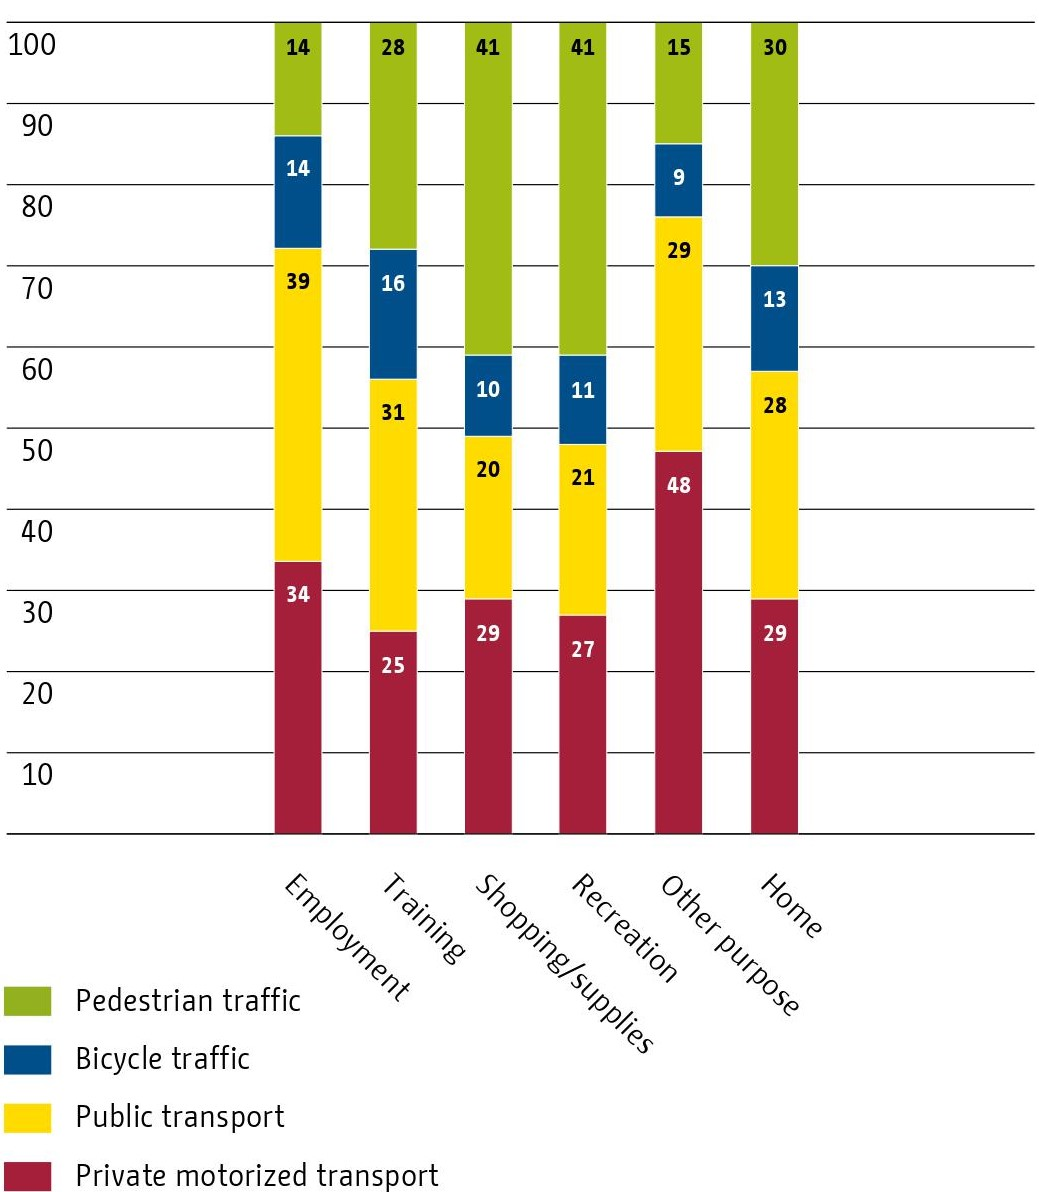
\includegraphics[width=0.5\textwidth]{MobilityInTheCityJPG/Graphs/UseOfTransportPurpose.jpg}
	\centering
	\caption{Use of transport mode by purpose of journey.\cite{MobilityCity}}
\end{figure}
\section{Car}

With a length of approximately 5400 km of roads the car remains the most used mean of transport to commute to work. Improving the roads and making more parking spaces available makes the car an atractive option. However, only 20\% of the road vehicles traveling in Berlin are private cars. The other 80\% cars are vehicles belonging to flexible, non-binding schemes and with a fixed pick-up point.  The main traffic roads\footnote{Main traffic roads: they have a total length of 160 km.} ensures that people coming from Berlin's suburbs or nearby cities reach the minor roads efficiently. The vast majority of these minor roads (370 km) have a speed limit of 30 km/h upon them, which is due to safety reasons and noise control\cite{MobilityCity}. 

The demand for parking spaces is significantly higher than the supply, but this is where Berlin's parking policy plays a big role. A 100,000 parking spaces across 45 parking zones provides a reasonable amount of place to store the commuters vehicle during day or night. Nevertheless parking in Berlin can get expensive. If you live in Berlin and you want to park in your neighbourhood you need a permit\footnote{In German: Bewohnerparkausweis} which costs \texteuro20.40 and is valid for two years. Otherwise you have to pay at the parking meter. Outside the \textit{Ringbahn}\footnote{Berliner Ringbahn: a 37.5 km long circle route around Berlin's inner area, on the Berlin S-Bahn network.} you can park for free. Other costs like car insurance (\texteuro100 to \texteuro1000 per year), vehicle tax\footnote{Kraftfahrzeugsteuer} (around \texteuro100 per year), fuel, avehicle inspections per two years (\texteuro100), maintenance and repairs make the use of the car for commuting an expensive option\cite{CostCars}.
\begin{figure}

	\begin{subfigure}[b]{.5\linewidth}
		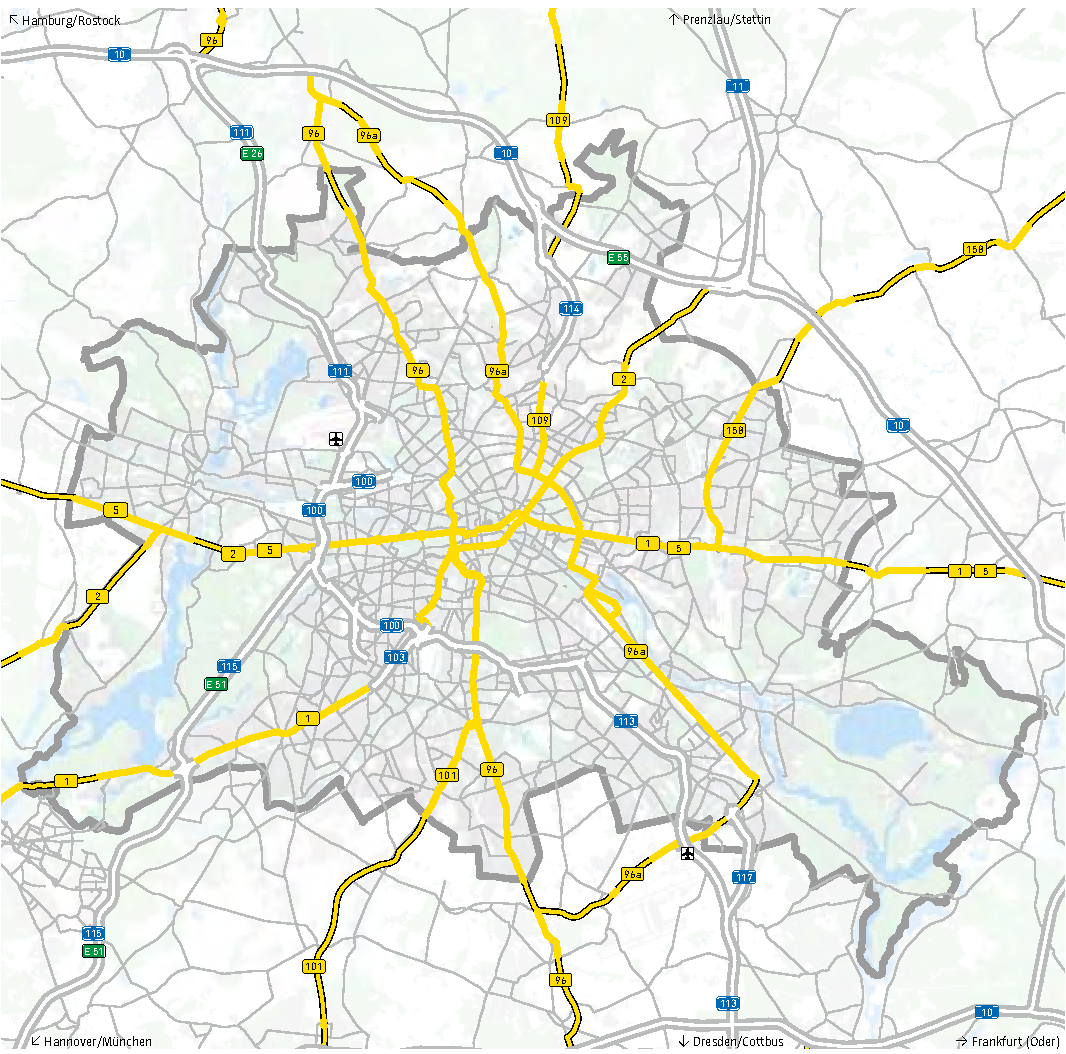
\includegraphics[width=\linewidth]{MobilityInTheCityJPG/Graphs/Motorways.pdf}
		\caption{Motorway and major road network}
		\label{Motorways}
	\end{subfigure}
	\begin{subfigure}[b]{.5\linewidth}
		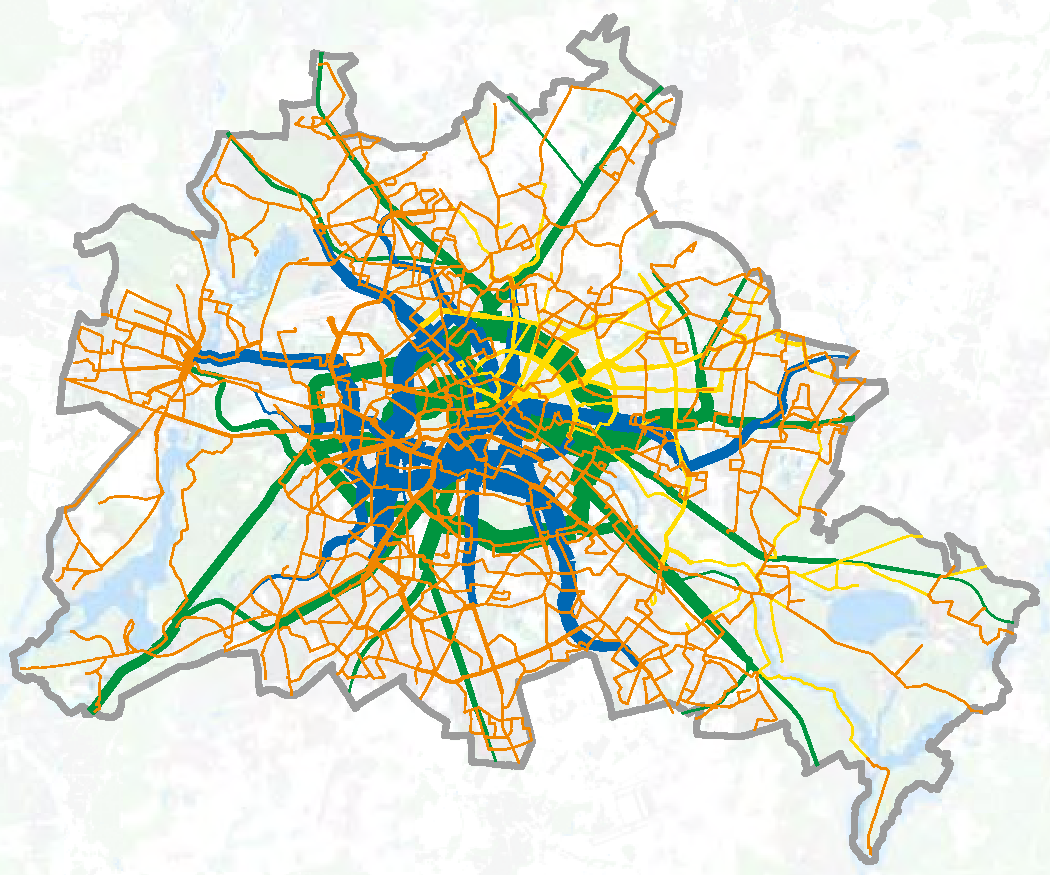
\includegraphics[width=\linewidth]{MobilityInTheCityJPG/Graphs/PTnetwork.pdf}
		\caption{Public transport network by transport mode}
		\label{PTnetwork}
	\end{subfigure}
\end{figure}


\section{Bus}

The bus network consists of a large network that covers almost the entire city of Berlin (orange lines in Figure \ref{PTnetwork}). The network consists of 149 daytime and 63 night bus routes, seventeen MetroBus and 13 express routes.  The day lines connect the suburbs with the central city or S-Bahn and U-Bahn stations. The night bus lines replace partially certain U-Bahn lines and the most important day lines. The MetroBuses give service in areas that are poorly served by the U-Bahn and S-Bahn. They are designated as part of the \textit{MetroNetz} and serve 24 hours per day, seven days per week, in intervals of ten minutes. The X-buses (express) are faster routes which is accomplished through a small number of the more important stops on the route. By the greater distance between the stops, the buses lose less time on stopping the vehicle\cite{xpress}. \\

\subsection*{BVG}
The \textit{Berliner Verkhersbetriebe} (BVG\footnote{BVG: An abbreviation from the original company \textit{\textbf{B}erliner \textbf{V}erkehrs-Aktien\textbf{g}esellschaft}}) is the main public transport company of Berlin. It coordinates and develops the U-Bahn, tram, bus, replacement services and ferry networks\cite{BVG1}. With their 3,000 vehicles, they transported 1,064 million passengers in 2016 or more than 2.7 million passengers per day\cite{MobilityCity}.


\section{Tram}
 The tram network in Berlin was founded in 1865 and is hereby one of the oldest there is. After Melbourne and St. Petersburg, it's the largest tram system in the world. Since 1929, the BVG has operated the system. It's made of 22 lines and measuring almost 190 km in route length. Also here there are nine Metrotrams that give service 24 hours per day with small intervals.

\section{Train}


\section{Ticketing system and price}


\section{Bike}


\section{Sharing systems}

